The learning process of a system begins by analyzing a \textit{trace} from a simulation.
%
A trace is a set of \textit{observations} from which \textit{equations} are derived, by fitting the trend of the data to mathematical functions.
%
Each equation represents a \textit{functionality} with knowledge to be incorporated into a \textit{learned model} as a \textit{node}. 
%
We use an \textit{incremental learning} approach, as each node to be incorporated is priorly \textit{measured} or evaluated in terms of cost with respect to the learned model.
%
Simultaneously, the structure of the learned model is matched against the one from the observed system, only to indicate the progress of the learning process. \\ \\
%
In this chapter we discuss how incremental learning works by first explaining how the data from observations is fitted to equations in the \textit{Data Fitting} section. Then we describe how the equations are used to learn information in section \textit{Data Learning}. We discuss how learned data is modeled in section \textit{Data Modelling}, and in the last section \textit{Cost Evaluation}, we explain how the use of costs influence the modelling and learning of data. 

\section{Data Fitting}
We consider an \textit{observation} as the value of a variable in an exact time, obtained from a simulation trace.
%
By gathering more than one observation and fitting the curve of the data, we are able to derive equations that express the  \textit{behavior} of a variable given a period of time. 
%
The procedure is implemented by storing the data of a trace using a \textit{buffer} (e.g. \ref{buffer_slide}) structure, that gathers observations from a simulation trace, which are later fitted to equations, as seen in algorithm \ref{dataFitter}. The buffer gathers observations, as long as the trace was not fully traversed (line number 2). The information of the \textit{buffer} was designed as a \textit{Map} in such way that the exact \textit{time} and \textit{value} of an observation can be extracted from it (lines 3-7). Once all observations were extracted from the \textit{buffer}, they are fitted and stored as equations in a list of equations (lines 8-9).
%
\begin{algorithm}
	\caption{Data-Fitter}
	\label{dataFitter}
	\begin{algorithmic}[1]
		\Procedure{fitdata}{timeStep, buffer, traceData}
		
		\While{$ windowSlideLimit == false $}
%		
%		\State $lastEquationFits \gets evaluateLastEquation(\vars{buffer})$
%		
%		\If{ $lastEquationFits = true$}
%			\State $updateLastEquationsConstraint(\vars{buffer})$
%		\Else
		
		\ForEach{$entry \in buffer $}
			\State $time\gets entry.getKey()$
			\State $value\gets entry.getValue()$
			\State $observations.add(time,value)$
		\EndFor
		
		\State $equation\gets \func{fitEquation}(\vars{observations})$
		\State $\func{equationsList.add}(\vars{equation})$
		
%		\EndIf
		
		\State $ windowSlideLimit \gets \func{slideBuffer}(\vars{timeStep, traceData})$
		
		\EndWhile
		
		\EndProcedure
	\end{algorithmic}
\end{algorithm}
	 
%
\begin{figure}[h]
\begin{center}
		\begin{tabular}{||c c ||}
		\hline
		Time & Value  \\ [0.5ex] 
		\hline\hline
		\textbf{0} & \textbf{1} \\ 
		\hline
		\textbf{1} & \textbf{2} \\
		\hline
		\textbf{2} & \textbf{3} \\
		\hline
		3 & 4 \\
		\hline
		4 & 5  \\ [1ex] 
		\hline
	\end{tabular}
	\begin{tabular}{||c c ||}
		\hline
		Time & Value  \\ [0.5ex] 
		\hline\hline
		 0 & 1 \\ 
		\hline
		\textbf{1} & \textbf{2} \\
		\hline
		\textbf{2} & \textbf{3} \\
		\hline
		\textbf{3} & \textbf{4} \\
		\hline
		4 & 5  \\ [1ex] 
		\hline
	\end{tabular}
	\begin{tabular}{||c c ||}
		\hline
		Time & Value  \\ [0.5ex] 
		\hline\hline
		0 & 1 \\ 
		\hline
		1 & 2 \\
		\hline
		\textbf{2} & \textbf{3} \\
		\hline
		\textbf{3} & \textbf{4} \\
		\hline
		\textbf{4} & \textbf{5}  \\ [1ex] 
		\hline
	\end{tabular}
\end{center}
\caption{Example of buffer storing information of a trace}
\label{buffer_slide}
\end{figure}

\section{Data Learning}
Given that each equation trace is organized by time and that the initial node of the learned model \textit{lm} is known.
%
For each equation in an equation trace, we proceed to traverse the learned model to measure the similarity between existing neighbor nodes or \textit{direct successors} and the observed equation. 
%
An equation is incorporated to the model depending on the distance that it has among the direct successors (if any), and the knowledge that we obtain from it, as seen in Algorithm \ref{learner}.
%
\begin{algorithm}
	\caption{Learner}
	\label{learner}
	\begin{algorithmic}[1]
		\Procedure{learner}{equationTrace}

			\State $parent \gets lm.getInitialLocation()$
			
			\ForEach {$equation \in equationTrace $}
			
				\State $directSuccessors \gets lm.getDirectSuccessors(\vars{parent})$
				
				\If{$directSuccessors.length>0$}
					\State $distances \gets \func{measureDistances(\vars{directSuccessors,equation})}$
					\State $lastModifiedNode \gets \func{incrementalLearning(\vars{distances})}$
				\Else
					\State $lastModifiedNode \gets \func{addNodeToLearnedModel(\vars{equation})}$
%					\State $Mark\_node\_as\_not\_learned$
				\EndIf
				
				\State $parent \gets \vars{lastModifiedNode}$
				
			\EndFor
			
		\EndProcedure
	\end{algorithmic}
\end{algorithm}


%
\subsection{Measuring Distance}
The similarity between direct successors and an observed equation is measured based on Euclidean distance with Algorithm \ref{measureDistances}. Given that \textit{time steps} represent the time range in which an equation was observed. For each \textit{neighbor} among the direct successors, we evaluate the fitted function of the observed equation \textit{observed function} and the one from the neighbor \textit{neighbor function} to obtain the two sets of points \textit{observed points} and \textit{neighbor points}, which will later be used to obtain the \textit{Euclidean distance}. It is important to note that the euclidean distance is normalized to a value between 0 and 1 in line 10 of the algorithm, and that we perform the same procedure for every neighbor and store every distance in the list \textit{distance list}. 
%
\begin{algorithm}
%	\caption{Get Distances. The distance is the euclidean distance between the values of the observed equation and a neighbor's equation, after both were evaluated with the time steps of the observed equation. 
%		\newline \textbf{Input}: Direct successors and an observed equation. 
%		\newline \textbf{Output}: List of the distance of all neighbors with respect to the observation. }
	\caption{Measure-Distances}
	\label{measureDistances}
	\begin{algorithmic}[1]
		\Procedure{measure-distances}{directSuccessors, observedEquation}
		
		\State $timeSteps\gets \vars{observedEquation.timeSteps}$
		\State $observedFunction\gets \vars{observedEquation.fittedFunction}$
		
		\ForEach {$neighbor \in directSuccessors$}
			\State $neighborFunction\gets \vars{neighbor.fittedFunction}$
			\State $neighborPoints \gets \func{evaluatefunction(\vars{neighborFunction, timeSteps})}$
			\State $observedPoints \gets \func{evaluatefunction(\vars{observedFunction, timeSteps})}$
			\State $distance \gets \func{getEuclideanDistance(\vars{observedPoints, neighborPoints})}$
			\State $distance \gets 1/(1+distance)$
			\State $distanceList.push(distance)$
		\EndFor
		
		\State \Return $distanceList$
	
		\EndProcedure
	\end{algorithmic}
\end{algorithm}



\section{Data Modelling}
We attempt to merge similar observations to avoid redundant or unnecessary nodes in our learned model, by using the gathered distances from Algorithm \ref{measureDistances}. 
%
Among all distances, we retrieve the node with the closest distance (\textit{closest node}) that satisfies our similarity criteria (\textit{similarity threshold}), with the intention of evaluating the cost of adding a similar observation as a \textit{new node} or as a \textit{merged node}. If an observation does not satisfy the similarity threshold, then the closest node below the threshold (\textit{far node}) is retrieved and added to the learned model as a new location. As depicted in Algorithm \ref{incrementalLearning}.
%
\begin{algorithm}
	\caption{Incremental-Learning. An observed equation is added to the learned model as a new node or as a merged node, based on the closeness that it has among direct successors.
	\newline Input: similarity threshold \textit{sim\_th}, given by the user}
%	\caption{Incremental-Learning}
	\label{incrementalLearning}
	\begin{algorithmic}[1]
		\Procedure{Incremental-Learning}{distances, observedEquation}
		
		\State $closestNode \gets \func{getClosestDistanceAboveThreshold(\vars{distances, sim\_th})}$
		\State $farNode \gets \func{getClosestDistanceBelowThreshold(\vars{distances, sim\_th})}$
		
		\If {closestNode.isNotEmpty()}
			\State $nextNode \gets \func{addLeastExpensiveChange(\vars{closestNode, observedEquation})}$
			\State	\Return $nextNodeToTraverse$
		\EndIf
		
		\If {farNode.isNotEmpty()}
			\State $nextNode \gets \func{addNodeToLearnedModel(\vars{farNode, observedEquation})}$
			\State	\Return $nextNode$
		\EndIf
	
		\EndProcedure
	\end{algorithmic}
\end{algorithm}



%
\section{Cost Evaluation}
%
The gathered knowledge of a system is always resembled by the latest structure and functionality of the learned model. An observed equation represents new knowledge, which we would like to incorporate to our learned model. The way that we evaluate this incorporation is by estimating the cost of the following points: Number of nodes required to express the information in the learned model (either as a new node or a replacement), plus the error that it may transmit or propagate to other relevant close nodes from the learned model, as seen in Equation \ref{cost}.
\begin{equation} 
\label{cost}
	Cost = nodeCount*nodeCost + propagation
\end{equation}
%
Based on the previous general cost function, we derive two types of cost functions to decide whether to add or replace nodes: \textit{replacement cost} and \textit{addition cost}, where we always conclude that the function with the lowest cost is the one that determines how an observed equation will be incorporated to the learned model. \\ \\
%
For explanation purposes, we will be making the following assumptions: 1) The Uppaal model from Figure \ref{learned_model_example} represents our learned model, 2) We have observed an equation $x=x+1$ from times \textit{0-10} of a simulation and wish to incorporate it to the model by utilizing cost functions. 
%
\begin{figure}[h]
	\centering
	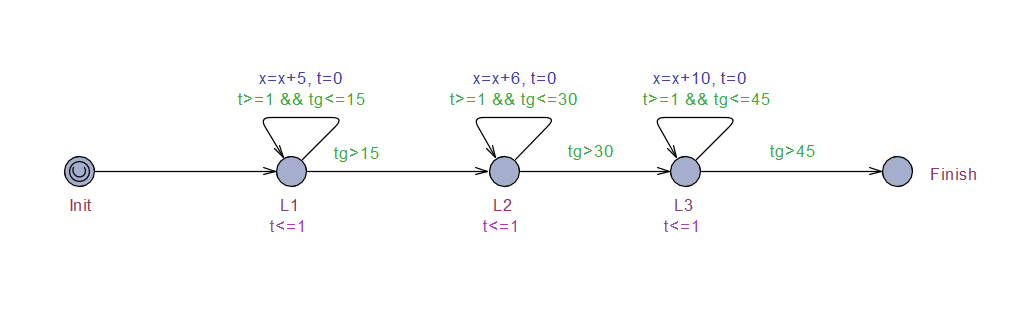
\includegraphics[scale=0.5]{./pictures/learned_model_example.png}
	\caption{Learned model example}
	\label{learned_model_example}
\end{figure}

\subsection{Addition Cost}
The addition of an observation consists of adding a node to the learned model without modifying other nodes functionalities and time constraints. The only cost for this change is determined by the \textit{addition cost}, thus the function cost for this case is determined by: $additionCost = nodeCost$. \\ \\
%
An example of adding the assumed observation as a new node to the learned model can be seen in Figure \ref{learned_model_example_addition}. 
%
\begin{figure}[t]
	\centering
	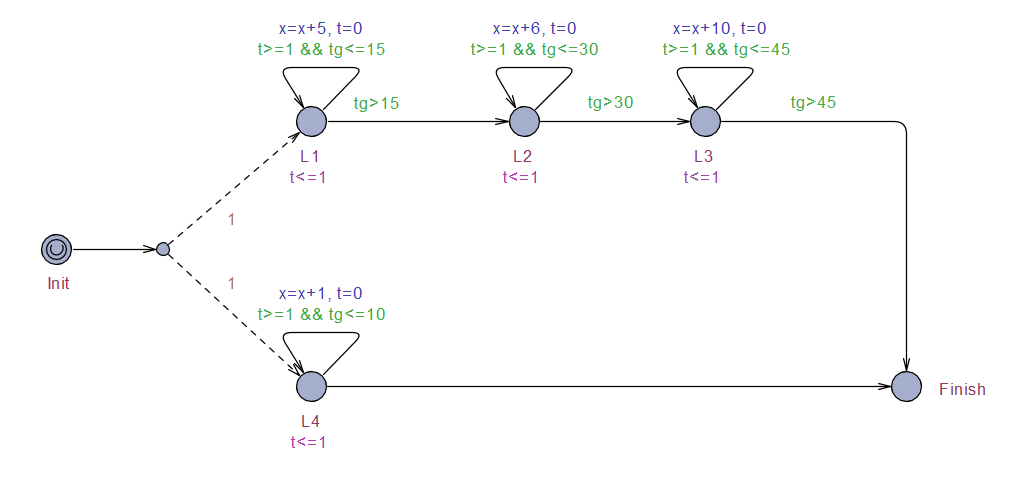
\includegraphics[scale=0.5]{./pictures/learned_model_example_addition.png}
	\caption{Node addition to learned model example}
	\label{learned_model_example_addition}
\end{figure}

\subsection{Replacement Cost}
The replacement of a node in the learned model consists of merging the functionality and time constraints of an observation with the ones from a node, without adding extra nodes. The cost of this change is mainly determined by two types of propagation:  functionality propagation ($propagation_f$) and time propagation ($propagation_t$):
%
\begin{equation}
replacementCost = propagation_f*functionalityCost + propagation_t* timeCost,
\end{equation}
where the first propagation represents how the modification of the functionality of a node can affect the distance of other nodes, while the second represents how modifying time constraints can affect other nodes. We will explain how location $L1$ is merged with the observation in the following subsections. 

\subsection{Time Propagation}
The already learned time constraints of $L1$ state that the location should be active for 15 seconds of the simulation and then take the edge to location $L2$. We have observed a functionality with a duration of 10 seconds (5 seconds less than $L1$). The possibilities of merging the time constraints of both the observation and $L1$ are given by the following cases:
\begin{itemize}
	\item Ignoring: We decide to ignore that we observed 5 seconds of the observation (e.g. times from 10 - 15) and not modify the time constraints of $L1$. 
	\item Updating: We decide to modify the time constraints of $L1$, as depicted in Figure \ref{learned_model_example_time_replacement}.
	\item Splitting: We decide to not modify the time constraints of $L1$ and add extra locations from the constraints that were not satisfied by $L1$. For this, we evaluate the time of the location $L1$ and the time of the observation $Obs$ as sets, and add locations according to the difference of the time sets. An example can be seen in Figure \ref{learned_model_example_time_replacement_addition})
%	\item Splitting: we decide to modify the time constraints of $L1$ and add a second location $L1'$, in which $L1$ will have the time constraints that satisfy the ones from  the observation and $L1'$ the ones that constraint that were not satisfied. 
%	  and penalize that we subtracted 5 times of activity of $L1$. 
\end{itemize}

\begin{figure}[h]
	\centering		
	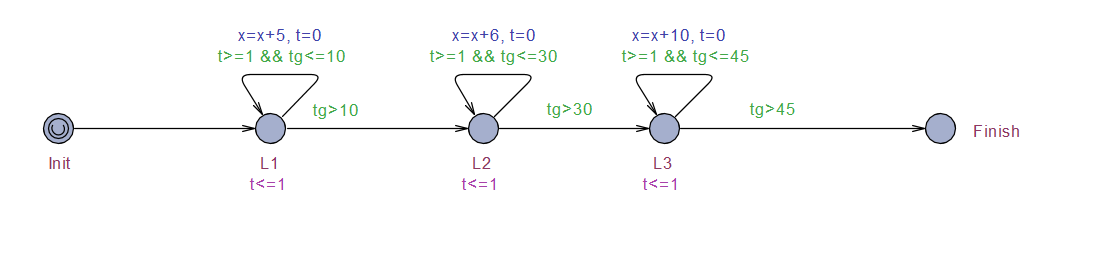
\includegraphics[scale=0.5]{./pictures/learned_model_example_time_replacement.png}
	\caption{Time constraints replacement in learned model example}
	\label{learned_model_example_time_replacement}
\end{figure}

\begin{figure}[h]
	\centering
	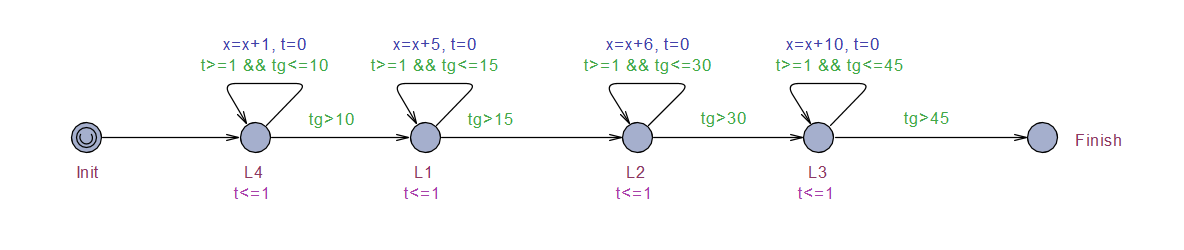
\includegraphics[scale=0.5]{./pictures/learned_model_example_time_replacement_addition.png}
	\caption{Time constraints replacement with extra location in learned model example}
	\label{learned_model_example_time_replacement_addition}
\end{figure}
%
%splitting case can be explained with a set. \\ \\
%
% Definition of circles
%\def\firstcircle{(0,0) circle (1.5cm)}
%\def\secondcircle{(0:2cm) circle (1.5cm)}
%
%\colorlet{circle edge}{blue!50}
%\colorlet{circle area}{blue!20}
%
%\tikzset{filled/.style={fill=circle area, draw=circle edge, thick},
%	outline/.style={draw=circle edge, thick}}
%
%\setlength{\parskip}{5mm}
%% Set A and B
%\begin{tikzpicture}
%\label{time_diagram}
%\begin{scope}
%\clip \firstcircle;
%\secondcircle;
%\end{scope}
%\draw[outline] \firstcircle node {$L1$};
%\draw[outline] \secondcircle node {$Obs$};
%\node[anchor=south] at (current bounding box.north) {Times analyzis};
%\end{tikzpicture}
%
%
For the first two cases, the $propagation_t$ cost is represented by the number of unseen times, which is 5, multiplied by the \textit{time cost}. The only time that the $propagation_t$ is zero, is in the last case when a location is added to keep the time constraints intact. Nevertheless, this last change causes the replacement cost to be raised by adding an additional location required to satisfy the observed time constraints. 

\subsection{Functionality Propagation}
Assuming that we want to merge the functionality of location $L1$ ($x=x+5$) with the observed functionality ($x=x+1$), we need to obtain a new fitted function. For this, we utilized the same fitting methodology as shown in Algorithm \ref{dataFitter}. We retrieve two sets of points by evaluating both functions in the same range of time and obtain the new fitted function (e.g. $x=x+3$). Once the new fitted functionality is replaced in $L1$, the $functionalityPropagation$ is determined by the difference of the Euclidean distance between the new functionality and the functionality of $L1$, along with the one from its direct successors. The result of the change  can be seen in Figure \ref{learned_model_example_time_replacement_functionality}. \\ \\
%
In this particular type of replacement, two aspects are considered:
\begin{itemize}
	\item Substitution: In this case we consider how close is the Euclidean distance of the new functionality compared to the one that was substituted. 
	\item Propagation: Here we perform the same comparison as in the previous case, but we now compare how the Euclidean distance of each direct neighbor is affected by the substituted location.
\end{itemize}
%
For the example in Figure \ref{learned_model_example_time_replacement_functionality}, we can clearly see that changing the functionality of location \textit{L1} from $x=x+5$ to $x=x+3$ has a negative effect, as the new functionality $x=x+3$ is distanced from $x=x+5$ and even more distanced from $x=x+6$. The main goal of this calculation is to consider how changing the functionality of a location can impact not only the location itself, but also others around it. 
\begin{figure}[h]
	\centering
	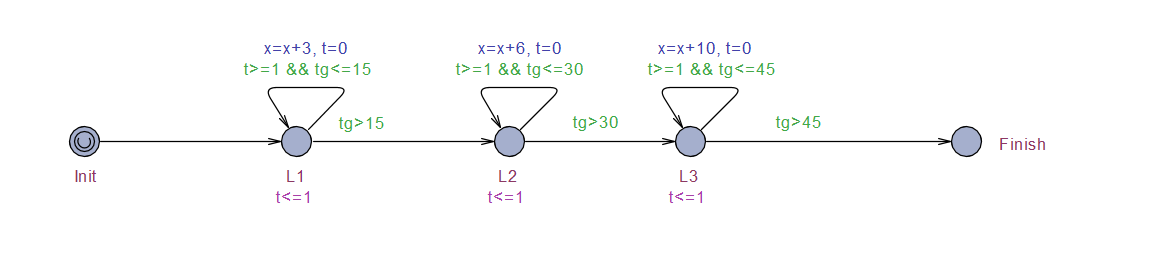
\includegraphics[scale=0.5]{./pictures/learned_model_example_replacement_functionality.png}
	\caption{Replacement of the functionality of a location in the learned model example}
	\label{learned_model_example_time_replacement_functionality}
\end{figure}

%learned_model_example_replacement_functionality

%\section{Graph Matching and Similarity Scoring}






